\section{Considerações inicias}
A organização de uma coleção de documentos em vários tópicos, de modo que exista sobreposição
entre os grupos é um importante problema em sistemas de recuperação de informação(SRIs). Na
literatura diversas estratégias são utilizadas visando otimizar a organização flexível de
documentos, conforme foi abordado no capítulo anterior. Soma-se a isso o fato de que a maioria dos
métodos que adicionam flexibilidade ao processo, como por exemplo  os métodos de agrupamento, nem
sempre são desenvolvidos com o foco em documentos textuais. Que conforme foi abordado ao longo do
texto, possui características que acrescentam algumas dificuldades no processo, tais como a alta
dimensionalidade dos dados, assim como também usualmente são armazenados de maneira não estruturada.
E ainda com o crescente aumento do uso de tecnologias de produção de conteúdo, a quantidade de dados
textuais alcança grandes volumes de dados o que os enquadra no contexto do $Big Data$. 
Portanto esse cenário fortalece a importância de se conduzir pesquisas e investigações em torno da
organização flexível de documentos. Entretanto não é esperado que um método de agrupamento seja
totalmente adequado para todos os tipos de dados, incluindo os dados de alta dimensionalidade como
os dados textuais\cite{Steinbach2004}. Desta maneira esse capítulo tem como objetivo detalhar as 
contribuições
desta monografia a organização flexível de documentos, através da investigação dos impactos de se
utilizar a estratégia de se misturar o agrupamento fuzzy e possibilístico provida pelo algoritmo
PFCM. Onde este método de agrupamento pretende resolver os problemas dos elementos equidistantes e 
dos grupos
coincidentes, apresentados nas partições fuzzy e possibilística respectivamente. 

Conforme observa-se no capítulo 2, o algoritmo PFCM produz duas
partições, sendo um fuzzy e outra possibilística, o que induziu o presente trabalho a propor duas extensões do
método de extração de descritores Soft-wFDCL proposto por \cite{Nogueira2013}, que leva em
consideração apenas os valores de pertinências presentes na partição fuzzy. A primeira extensão
denominada Mixed-PDCL({\it Mixed - Possibilistic Fuzzy Descriptor Comes Last\/}), 
a qual contempla durante a extração de descritores as duas partições do PFCM.
E a segunda proposta é o método 
MixedW-PDCL({\it Mixed Weighted - Possibilistic Fuzzy Descriptor Comes Last\/}), 
que é uma extensão do Mixed-PDCL, porém ponderando as
contribuições das partições com base nos parâmetros $a$ e $b$ do PFCM. A última contribuição é a
proposta do método HPCM, que é uma extensão do método de agrupamento hierárquico HFCM, o qual
utiliza o algoritmo PCM no lugar do FCM para produzir a hierarquia.

Na primeira sessão deste capítulo é apresentado informações das bases de dados utilizadas, com as
suas características, origem e composição dos documentos. Nos capítulos seguintes é definido as
propostas sugeridas por essa monografia. E por fim os dados obtidos com os experimentos realizados.

\section{Informações das bases de dados}

Na mineração de dados e consequentemente nos trabalhos relacionados a organização flexível de
documentos, é comum se realizar a avaliação dos métodos propostos, conduzindo-se experimentos sobre
bases de dados existentes na literatura com essa finalidade\cite{Rossi2013}. Para isso, as bases
precisam estar apresentadas de maneira estruturada. Assim sendo, nesta pesquisa foi adotado o formato
{\it tf-idf\/}(\ref{eq:tfidf}) como forma de estruturar os dados presentes nas bases, 
de modo a capturar a
importância relativa dos termos nos documentos e na coleção. Cada coleção foi então disposta em dois
arquivos, sendo que o arquivo com extensão $.data$ contém $n$ linhas, onde cada linha constitui a 
representação de um
documento da coleção no formato {\it tf-idf\/}, para $n$ igual a quantidade de documentos 
presentes na
coleção, enquanto o que arquivo de extensão $.names$ possui a descrição dos $m$ termos existentes na
coleção dispostos um por linha.

A base Opinosis\footnotemark é composta de opiniões de consumidores a respeito das características de alguns
produtos, obtidas dos portais amazon.com, tripadvisor e edmunds.com. As opiniões presentes na base,
abordam tópicos como serviços de hospedagem, dispositivos eletrônicos e carros. Sendo que no total
as sentenças presentes na coleção estão distribuídas em 51 categorias, onde cada categoria possui
100 sentenças na média. Os dados dessa base
foram obtidos no repositório {\it UCI Machine Learning Repository\/}\cite{Frank2010}, 
que mantém várias coleções de
dados que são utilizados pela comunidade de aprendizado de máquina para a realização de análises
empíricas dos algoritmos.
\footnotetext{\url{http://archive.ics.uci.edu/ml/datasets/Opinosis+Opinion+26frasl3B+Review}}

A coleção de documentos 20Newsgroup\footnotemark original contém aproximadamente 20000 documentos de notícias,
particionados em mais ou menos 20 temas. No entanto para os experimentos realizados nesta pesquisa, 
foi utilizado uma versão mais
compacta da coleção, contendo 2000 documentos pertencentes ao tema ciência, a qual contém os tópicos
sci.space, sci.electronics e sci.med. Esta base tem-se mostrado bastante popular em
aplicações textuais de aprendizado de máquina\cite{Nogueira2015}, tais como agrupamento e 
classificação de textos.
Essa base foi coletada originalmente por Ken Lang para a pesquisa Newsweeder apresentada em
\cite{Lang1995}. 
\footnotetext{\url{http://qwone.com/~jason/20Newsgroups/}}

Os documentos presentes na base de dados Reuters-21578\footnotemark apareceram inicialmente na Reuters newswire
em 1987. Sendo que os documentos foram coletados e indexados diretamente por membros da Reuters e da
{\it Carnegie Group, Inc.} também em 1987 para o desenvolvimento do CONSTRUE\cite{Hayes1990}, que
foi um sistema de categorização de documentos. Onde no ano de 1990 essa base de dados foi tornada
pública pela Reuters, para ser utilizada em pesquisas de recuperação de informação. No entanto as
versões inicias dessa base continham documentos repetidos e ambíguos, o que motivou um grupo de
pesquisadores de categorização textual durante a conferência {\it ACM SIGIR '96\/}, a realizar uma
limpeza na base, possibilitando uma melhor comparação dos resultados entre diferentes estudos. Essa
versão final ficou com o total de 21578 documentos, distribuídos entre 43 diferentes categorias. 
Contudo
nesta pesquisa foi utilizada uma amostragem menor da coleção, contendo 1052 documentos, selecionados
aleatoriamente de cada classe da coleção.
\footnotetext{\url{https://archive.ics.uci.edu/ml/datasets/Reuters-21578+Text+Categorization+Collection}}

A base de dados WAP({\it WebACE Project\/}) é composta de um conjunto de páginas web coletadas por 
\citeonline{Moore1997}, para um projeto de pesquisa de agrupamento, seleção e recuperação de páginas web.
Os dados presentes nesta coleção foram obtidos pelos autores do artigo em 98 páginas web, onde
posteriormente foram distribuídos em 20 diferentes categorias, que abrangem tópicos como negócios e 
finanças, tecnologias, trabalho e
indústria. O conteúdo obtido está disposto em 1560 documentos na sua versão original, sendo que
todos os documentos foram utilizados nessa pesquisa.

A coleção de documentos NSF\footnotemark({\it National Science Foundation\/}) foi obtida do 
repositório de dados para pesquisas de aprendizado de máquina 
{\it UCI Machine Learning Repository}\cite{Frank2010}. O conteúdo dos dados presentes na base é
composto de 129000 resumos, sendo um resumo por documento, descrevendo prêmios da NSF para 
pesquisas básicas. Para os experimentos descritos nesta monografia, foram selecionados 1600 
documentos de maneira aleatória entre as categorias apresentadas na coleção.
\footnotetext{\url{https://archive.ics.uci.edu/ml/datasets/NSF+Research+Award+Abstracts+1990-2003}}

A base de dados Hitech adquirida em \citeonline{Karypis2006}, é parte de uma coleção de bases da 
conferência TREC({\it Text REtrieval Conference\/})\footnotemark. 
\footnotetext{\url{http://trec.nist.gov/data.html}}
Esta base é composta de um conjunto de notícias da revista {\it Jose Mercury News\/}\footnotemark, 
as quais são distribuídos em categorias distintas. As notícias presentes na coleção
abordam temas como computadores, eletrônicos, saúde, medicina, pesquisa e tecnologia. 
A base originalmente possui 2301
documentos, onde para esta pesquisa foram selecionados uma amostragem aleatória contendo 600
documentos. 
\footnotetext{\url{http://www.mercurynews.com/}}

\begin{table}[!htp]
  \centering
  \begin{tabular}{ |c|p{11cm}|}
    \hline
    {\bf documentos} & número de documentos presentes na coleção \\
    \hline
    {\bf termos} & número de termos existentes na coleção após o pré-processamento \\
    \hline
    {\bf \% zeros} & número relativo de zeros na {\it tf-idf\/}, ou seja quantifica o quanto a
matriz é esparsa \\
    \hline
    {\bf classes} & número de classes presentes na coleção \\
    \hline
    {\bf dp-class} & desvio padrão ao se considerar o percentual de documentos que
pertence a determinada classe na coleção \\
    \hline
    {\bf $>$classe} & percentual de documentos pertencentes a maior classe na coleção \\
    \hline
    {\bf n-gramas} & quantidade de termos considerados sequencialmente na coleção \\
    \hline
  \end{tabular}
  \caption{Descrição das características objetivas presentes em coleções textuais elencadas para
este trabalho}
  \label{table:datainfo}
\end{table}

Outro aspecto não menos importante, são as características particulares das coleções de dados. Pois
ressalta-se que para uma mais apurada análise dos resultados, é pertinente considerar as
particularidades de cada base, com a finalidade de encontrar possíveis justificativas para os
resultados apresentados, realizando-se indagações comparativas as peculiaridades sabidamente
conhecidas dos métodos analisados. Portanto o conjunto de características particulares de cada base
obtidos em \citeonline{Rossi2013} e adaptados a esta pesquisa, dar-se à como apresentado
na Tabela (\ref{table:datainfo}). 


Portanto, uma análise objetiva das características presentes nas seis bases descritas anteriormente 
está apresentado na (\ref{table:datasets}). Onde é possível notar de maneira bem 
objetiva ao se observar
a coluna \% zeros da tabela, que todas as bases apresentam uma quantidade de zeros em mais de $90\%$
dos dados, o que caracteriza o peculiar problema dos dados esparsos já caracterizado ao longo do
texto, como algo inerente aos dados textuais.


\begin{table}[!htp]
  \centering
  \begin{tabular}{ |l|c c c c c c c|}
    \hline
    {\bf nome} & docs & termos & classes & \% zeros & dp-classe & $>$classe & n-gramas \\
    \hline
    {\bf Opinosis} & 51 & 842 & 3 & 95,73\% & 0,1 & 96,07\% & 1-grama \\
    \hline
    {\bf 20newsgroups} & 2000 & 11028 & 4 & 99,11\% & 0,1 & 25\% & 1-grama \\
    \hline
    {\bf Hitech} & 600 & 6925 & 6 & 97,93\% & 0,1 & 16,67\% & 1-grama \\
    \hline
    {\bf NSF} & 1600 & 2806 & 16 & 99,76\% & 0,1 & 3,12\% & 1-grama \\
    \hline
    {\bf WAP} & 1560 & 8070 & 20 & 98,51\% & 0,1 & 100\% & 1-grama \\
    \hline
    {\bf Reuters-21578} & 1052 & 3925 & 43 & 98,55\% & 0,1 & 8,55\% & 1-grama \\
    \hline
  \end{tabular}
  \caption{Características das bases de dados utilizadas nesta pesquisa}
  \label{table:datasets}
\end{table}

\section{Refinamento com o algoritmo PFCM}

Conforme ficou evidenciado, a tarefa de organizar de maneira flexível um conjunto de documentos
textuais, possui diversos desafios. Em particular, ao se agrupar um conjunto de documentos é
esperado que os grupos resultantes possuam significado relevante, ou seja o algoritmo de
agrupamento precisa detectar a estrutura natural dos dados\cite{Steinbach2004}. Alguns desses 
desafios está na dificuldade em escalar os métodos usuais para bases de dados na categoria {\it Very Large}
conforme a escala apresentada na Tabela \ref{table:datasize}, assim como também a obtenção de
mecanismos efetivos para se avaliar a qualidade dos grupos produzidos, técnicas para se medir a
interpretabilidade dos resultados, capacidade para estimar os parâmetros dos algoritmos,
possibilidade para funcionar de maneira incremental, reduzindo o custo computacional durante a
atualização dos grupos com novos dados, e também a capacidade de continuar a produzir bons
resultados em cenários compostos de documentos ruidosos \cite{Carvalho2016}. 

Portanto para \citeonline{Steinbach2004}:
\begin{citacao}
  {\it [...] there is no reason to expect that one type of clustering approach will
  be suitable for all types of data, even all high dimensional data. Statisticians and other
  data analysts are very cognizant of the need to apply different tools for different types of
  data, and clustering is no different\/}.
\end{citacao}

Diante então dos desafios propostos, e com a evidência de que é possível aprimorar os resultados, ao
se utilizar novas estratégias de agrupamento. A investigação apresentada nesta seção tem como
objetivo analisar de qual forma a organização de documentos pode ser otimizada, ao aplicar na etapa
de agrupamento uma estratégia que misture as partições possibilística e fuzzy, através do algoritmo
PFCM. A escolha desse algoritmo foi feita devido o seu potencial para absorver as qualidades
presentes no FCM contrabalanceando as suas deficiências ao agregar também o PCM e sua partição
possibilística. Outro ponto a se considerar são as diversas pesquisas na literatura abordando o
desempenho do PFCM, 
como por exemplo em \citeonline{Pal2005,Yan2009,Kumar2010,Grover2014,Popescu2015}.

Com isso foi conduzido um experimento adaptando a estratégia de organização flexível de documentos
definida em \citeonline{Nogueira2013},
utilizando na etapa de agrupamento o método PFCM. Porém esse método produz duas partições uma
possibilística e uma partição fuzzy. Desse modo foi aplicado o método de extração de descritores
Soft-wFDCL na partição fuzzy e outra vez na partição possibilística, produzindo assim dois grupos de
descritores. Essa adaptação está ilustrada na Figura (\ref{fig:flexibleorganization}).

\begin{figure}[!htp] 
  \centering
  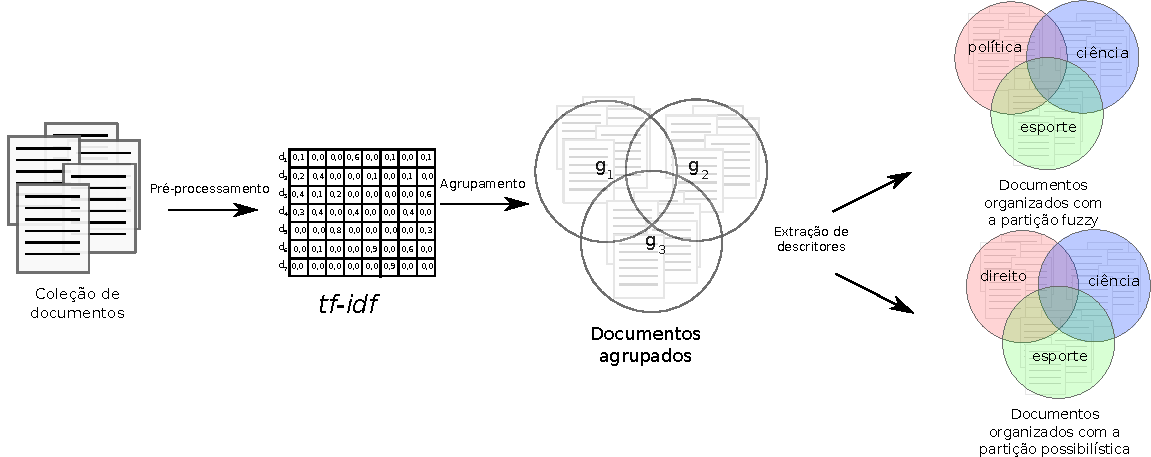
\includegraphics[width=1.0\columnwidth]{assets/process_pfcm.pdf} 
  \caption{Estratégia de organização flexível de documentos} 
  \label{fig:flexibleorganization} 
\end{figure}


\section{Método Mixed-PDCL}
\section{Método MixedW-PDCL}
\section{Método HPCM}
\section{Considerações finais}
